\section{Heating and Cooling in HII regions}

\lstinputlisting[caption={Code for the root finding algorithms}, firstline={247}]{ancillary.py}
\lstinputlisting[caption={Setup code for the second assignment}, linerange={19-35}]{hii_regions.py}

In this section we will investigate the equilibrium temperature of heating and cooling rates in an HII region similar to Orion. We will search for these equilibrium temperatures using a root finding algorithm. In this work we have chosen to use a combination of the False Position (FP) and Raphson-Newton (RN) methods to combine the guaranteed convergence of FP with the speed and accuracy of RN. We do this by first applying a broad bracket around the root and use FP to approach the root up to an accuracy $\epsilon_{FP}$ (step size along the x-axis, or relative y-accuracy). We have set $\epsilon_{FP} = 10^{-5}$ experimentally, as for higher values the algorithms tend to converge, and for lower values convergence time quickly approaches that of only using FP. Once the False Position algorithm has reached $\epsilon_{FP}$ we give the current best estimate to the Rapshon-Newton algorithm until it converges below our target accuracy.

\subsection{Simple Case}

First we will only consider an HII region with one heating and cooling mechanism. The heating is produced by photoionization given by

\begin{equation}
    \Gamma_{pe} = \alpha_B n_H n_e \psi k_B T_c,\label{eq:gamma_pe}
\end{equation}

and the cooling through radiative recombination:

\begin{equation}
    \Lambda_{rr} = \alpha_Bn_Hn_e\left<E_{rr}\right>,\label{eq:lamda_rr}
\end{equation}

with

\begin{equation}
    \left<E_{rr}\right> = \left[0.684 - 0.0416\ln\left(\frac{T_4}{Z^2}\right)\right]k_BT.
\end{equation}

In these equations, $\alpha_B = 2 \times 10^{-13}$ cm$^3$ s$^{-1}$ is the case B recombination coefficient, $k_B = 1.38\times 10^{-16}$ erg K$^{-1}$ is the Stefan-Boltzmann constant, $\phi = 0.929$ is given, $T_c = 10^4$ K is the stellar temperature, $Z = 0.015$ is the metalicity and $T_4 \equiv \frac{T}{10^4\text{K}}$ is the temperature. Finally, we assume the proton and electron densities to be equal, such that $n_e = n_p$.

The equilibrium temperature $T_eq$ is given by the temperature at which the heating rate is equal to the cooling rate, $\Gamma_{pe} = \Lambda_{rr}$. We can formulate this in terms of a root finding problem by searching for the point where $\Gamma_{pe} - \Lambda_{rr} = 0$. We can work out what this should be by combining equations \ref{eq:gamma_pe} and \ref{eq:lamda_rr} to find that this means the following should hold

\begin{equation}
    \psi T_c - \left[0.684 - 0.0416\ln\left(\frac{T}{10^4\cdot Z^2}\right)\right] \cdot T = 0.
\end{equation}

Note that the densities $n$, $\alpha_B$ and $k$ have all dropped out of this specific equation, even though this does not represent the true difference between heating and cooling rate at other temperatures. This is not important because we are only interested in the temperature at which the above equation is true, where additional scaling factors are important.

We apply our root finding algorithm introduced earlier to this equation with an initial bracket in the range $T = \left[1, 10^7\right]$ K. We aim for a temperature accuracy of $0.1$ K. We present the result in figure \ref{fig:simple_roots}, we can see that we find a root at $T = 3.25 \times 10^4$ K, where the function has a value of exactly $0$. It is a little bit strange that this value is exactly zero as we would expect some very small number, but not precisely zero. Most likely the algorithm came so close to the root that it arrived in the range of round-off errors and set the function value to $0.0$. The root finding algorithm on this function converged in 15 iterations, taking $\sim 1 \times 10^{-4}$ s (see terminal).


\begin{figure}
    \centering
    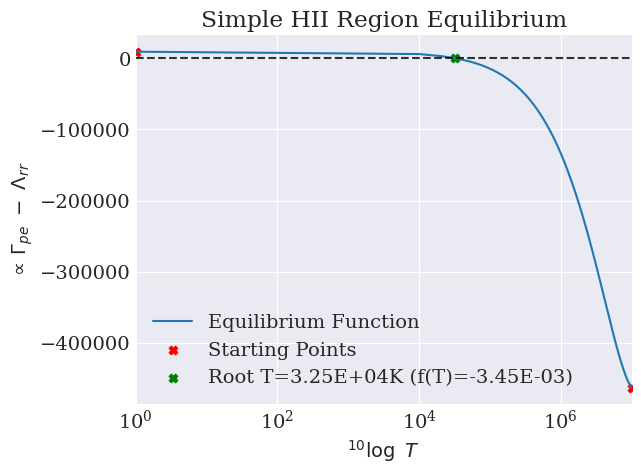
\includegraphics[width=0.8\textwidth]{results/simple_hiiregion_roots.png}
    \caption{The balance between the photoionization heating effect and radiative recombination cooling effects plotted as a function of temperature, combined with its root as determined using the FP-NR algorithm described at the beginning of this section. The values on the y-axis do not represent true values as they are off by multiple scaling factors as described in text.}
    \label{fig:simple_roots}
\end{figure}

\lstinputlisting[caption={Code for the simple equilibrium case root finding}, linerange={37-62}]{hii_regions.py}

\subsection{More Complex Case}

In addition to the singular heating and cooling mechanisms we described in the previous section, we will now setup a more realistic scenario and also include cooling through free-free emission ($\Lambda_{ff}$) and heating through cosmic rays ($\Sigma_{cr}$) and magnetohydrodynamic waves ($\Sigma_{MHD}$). These are all individually,given by the following three equations:

\begin{equation}
    \Lambda_{ff} = 0.54 T_4^{0.37}\alpha_Bn_en_hk_BT
\end{equation}
\begin{equation}
    \Gamma_{cr} = An_e\xi_{CR} \\
\end{equation}
\begin{equation}
    \Gamma_{MHD} = 8.9 \times 10^{-26}n_hT_4
\end{equation}

Synonymous to the previous section we can find the equilibrium temperature $T_{eq}$ by finding the temperature for which $\Gamma - \Lambda = 0$ where $\Gamma$ and $\Lambda$ represent the total heating and cooling rate respectively, which are just the sums of each of the individual effects. Working this out, we find that the following equation most hold:

\begin{align}
    \bigg(\psi T_c - \left[0.684 - 0.0416\left(\frac{T}{10^4\cdot Z^2}\right)\right] \cdot T &- 0.54 \left(\frac{T}{10^4}\right) T \bigg)\cdot k_Bn_H\alpha_B\nonumber \\
    ... &+ A\xi + 8.9 \times 10^{-26}n_H\frac{T}{10^4} = 0\label{eq:equi2}
\end{align}

We are going to attempt to find the equilibrium temperatures for three different cases where we vary the density from low to high. Specifically, we will take $n= [10^{-4}, 1, 10^4]$ cm$^{-3}$. We apply the same method as in the previous section, but in the figure we plot $^{10}\log|\Gamma~-~\Lambda|$ on the y-axis instead. We have to do this due to the different scales of the function at different densities. Plotting it like this also more directly highlights the root of the function as a sharp spike downwards. This happens because as the function goes to zero, its log goes to $-\infty$. We would therefore expect our root finding algorithm to place its root at these throughs.

We present the results of our root finding algorithm visually in figure \ref{fig:complex_roots} and numerically in table \ref{tab:complex_roots}, there we also provide the number of iterations and time taken for convergence. Note that this time is only a rough estimate as the algorithms were only run once to obtain this, however we see that execution time remains relatively constant in different runs. In the figure we can clearly see that this is the case, which indicates that our root finding algorithm has properly identified the equilbrium temperatures.

\begin{figure}
    \centering
    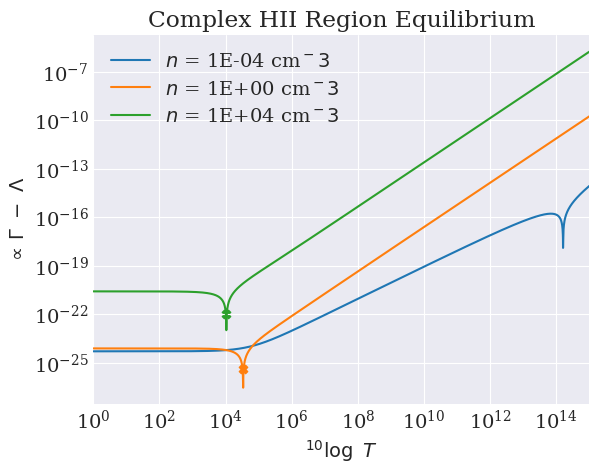
\includegraphics[width=0.8\textwidth]{results/complex_hiiregion_roots.png}
    \caption{The balance between all heating and cooling effects plotted as a function of temperature, combined with its root as determined using the FP-NR algorithm described at the beginning of this section for three different gas densities ($n = [10^{-4}, 1, 10^4]$ cm$^{-3}$). The y-axis represents the log of the absolute value of the difference between the heating and cooling mechanisms. We have plotted them this way to better visualize all three curves simultaneously. The deep throughs correspond to the roots of the function as described in the text.}
    \label{fig:complex_roots}
\end{figure}


\begin{table}[h]
    \centering
    \begin{tabular}{c|c|c|c|c}
        $n$ [cm$^{-3}$] & $T_{eq}$ [K] & $f(T_{eq})$ & Num Iterations & Elapsed Time [s] \\
        \hline
        \input{results/complex_hiiregion_table.txt}
    \end{tabular}
    \caption{Results of the FP-NR root finding algorithm on equation \ref{eq:equi2} for three different densities. The elapsed time is only measured once, but provides a rough estimate of execution time for each density.}
    \label{tab:complex_roots}
\end{table}

We can see that for the very low density gas ($n=10^{-4}$ cm$^{-3}$), the temperature required to reach an equilibrium between heating and cooling is extremely large, $T_{eq} = 1.61\times 10^{14}$ K. For comparison, the effective temperature of our sun is only $T_{eff} = 5.8 \times 10^3$ K. If we increase the density the required equilbrium temperature appears to drop $\sim$10 orders of magnitude to $T \sim 10^4$ K. From these three data points it appears that increasing the density above $1$ cm$^{-3}$ has little effect on the equilibrium temperature.

\lstinputlisting[caption={Code for the more complex equilibrium case root finding}, linerange={64-93}]{hii_regions.py}
